%!Tex Program = xelatex
\documentclass[10pt,a4paper,fleqn]{article}
\usepackage{fontspec, xunicode, xltxtra}
%\usepackage{xeCJK}
\usepackage[slantfont,boldfont]{xeCJK} % 允许斜体和粗体
\usepackage{multirow}
\usepackage{multicol}
\usepackage{titlesec}
\usepackage{enumerate}
\usepackage{booktabs}
\usepackage[table,xcdraw]{xcolor}
\usepackage{float}
\usepackage{geometry}
\usepackage{tikz}
\usepackage{tikz-qtree}
\usepackage{amsmath,amssymb}
\usepackage{extarrows}
\usepackage[colorlinks,linkcolor=black]{hyperref}
\usepackage{zhnumber}
\usepackage{listings}
\usepackage{pdfpages}
\usepackage{dirtree}

\geometry{left=2.5cm,right=2.5cm,top=2cm,bottom=2cm}

%cmd “fc-list :lang=zh-cn”
%\defaultfontfeatures{Mapping=tex-text}
\setmainfont{Book Antiqua}   % 英文衬线字体 Times New Roman, Palatino Linotype
\setmonofont{Consolas}   % 英文等宽字体 Monaco
\setsansfont{Consolas} % 英文无衬线字体 Arial, Futura, Optima
\setCJKmainfont{SimSun}   % 设置缺省中文字体
\setCJKmonofont{FangSong}   % 设置等宽字体
\setCJKsansfont{SimHei}   % 设置无衬线字体 Microsoft YaHei

\newfontfamily\timesroman{Times New Roman}
\newfontfamily\consolas{Consolas}

\newfontfamily\ensong{SimSun}
\newfontfamily\enhei{SimHei}
\newfontfamily\enyahei{Microsoft YaHei}
\newfontfamily\palatino{Palatino Linotype}
\newfontfamily\nimbus{Nimbus Sans L}
\newfontfamily\enkai{KaiTi}
\newfontfamily\enfangsong{FangSong}
\newfontfamily\enstzhsong{STZhongsong}
\newfontfamily\enstsong{STSong}

\setCJKfamilyfont{song}{SimSun}
\newcommand{\song}{\CJKfamily{song}}
\setCJKfamilyfont{heiti}{SimHei}
\newcommand{\heiti}{\CJKfamily{heiti}\enhei}
\setCJKfamilyfont{yahei}{Microsoft YaHei}
\newcommand{\yahei}{\CJKfamily{yahei}\enyahei}
\setCJKfamilyfont{kaiti}{KaiTi}
\newcommand{\kaiti}{\CJKfamily{kaiti}\enkai}
\setCJKfamilyfont{fangsong}{FangSong}
\newcommand{\fangsong}{\CJKfamily{fangsong}\enfangsong}
\setCJKfamilyfont{stzhsong}{STZhongsong}
\newcommand{\stzhsong}{\CJKfamily{stzhsong}\enstzhsong}
\setCJKfamilyfont{stsong}{STSong}
\newcommand{\stsong}{\CJKfamily{stsong}\enstsong}

\XeTeXlinebreaklocale "zh"
\XeTeXlinebreakskip = 0pt plus 1pt minus 0.1pt

%------------------------------标题名称中文化-----------------------------%
\renewcommand\abstractname{\heiti 摘\ 要}
\renewcommand\refname{\scriptsize 参考文献}
\renewcommand\figurename{\scriptsize 图}
\renewcommand\tablename{\scriptsize 表}

%\titlespacing*{\chapter} {0pt}{50pt}{40pt}
%\titlespacing*{\section} {0pt}{3.5ex plus 1ex minus .2ex}{2.3ex plus .2ex}
%\titlespacing*{\subsection} {0pt}{3.25ex plus 1ex minus .2ex}{1.5ex plus .2ex}
%\titlespacing*{\subsubsection}{0pt}{3.25ex plus 1ex minus .2ex}{1.5ex plus .2ex}
%\titlespacing*{\paragraph} {0pt}{3.25ex plus 1ex minus .2ex}{1em}
%\titlespacing*{\subparagraph} {\parindent}{3.25ex plus 1ex minus .2ex}{1em}

\titleformat{\section}{\bf\song}{\zhnumber{\thesection}、}{0em}{}
\titleformat{\subsection}{\bf\song}{\thesubsection}{0.5em}{}

%\setlength{\baselineskip}{1em}
\setlength{\parindent}{2em}
\setlength{\parskip}{0.2\baselineskip}
\setlength{\abovedisplayskip}{0.5pt}
\setlength{\belowdisplayskip}{0.5pt}

\newcommand{\hangpar}{\par\noindent\hangafter=1\setlength{\hangindent}{2em}}

\aboverulesep=0pt
\belowrulesep=0pt

\lstset{
    language=verilog,
    basicstyle=\small,
    numbers=left,
    numberstyle=\small,
    stepnumber=1,
    numbersep=5pt,
    backgroundcolor=\color{white},
    %keywordstyle=\color{keywordcolor}\bfseries, %\underbar,
    keywordstyle=\color{blue}\bfseries,
    morekeywords={*,\$write},
    identifierstyle=\small,
    showspaces=false,
    showstringspaces=false,
    showtabs=false,
    tabsize=4,
    frame=single,
    commentstyle=\color{olive} \textit,
    stringstyle=\ttfamily,
    showstringspaces=false,
    captionpos=b,
    breaklines=true,
    breakatwhitespace=true,
  }

\lstdefinelanguage{Assembler} {
  numberblanklines=false,
  keywordstyle=\color{blue}\bfseries,
  morekeywords={nop,halt,load,ld,store,str,ldih,mov,
  add,addi,addc,sub,subi,subc,cmp,
  and,or,xor,not,sl,sll,sla,srl,sra,
  j,jump,jmpr,jr,bz,bnz,bn,bnn,bc,bnc},
  morecomment=[l]{\#},
}

\lstdefinelanguage{PlainText} {
  numberblanklines=false,
}

\begin{document}
  \begin{center}
  \stzhsong
  \LARGE{中山大学本科生实验报告}\\[10pt]
  \Large{(2016学年春季学期)} \\[20pt]
  \end{center}
  \begin{flushleft}
    \stsong
    课程名称:嵌入式系统案例分析与设计
    \hspace{3em}
    任课教师:  {\bf 王军}
    \hspace{3em}
    助教:杨涵铄
    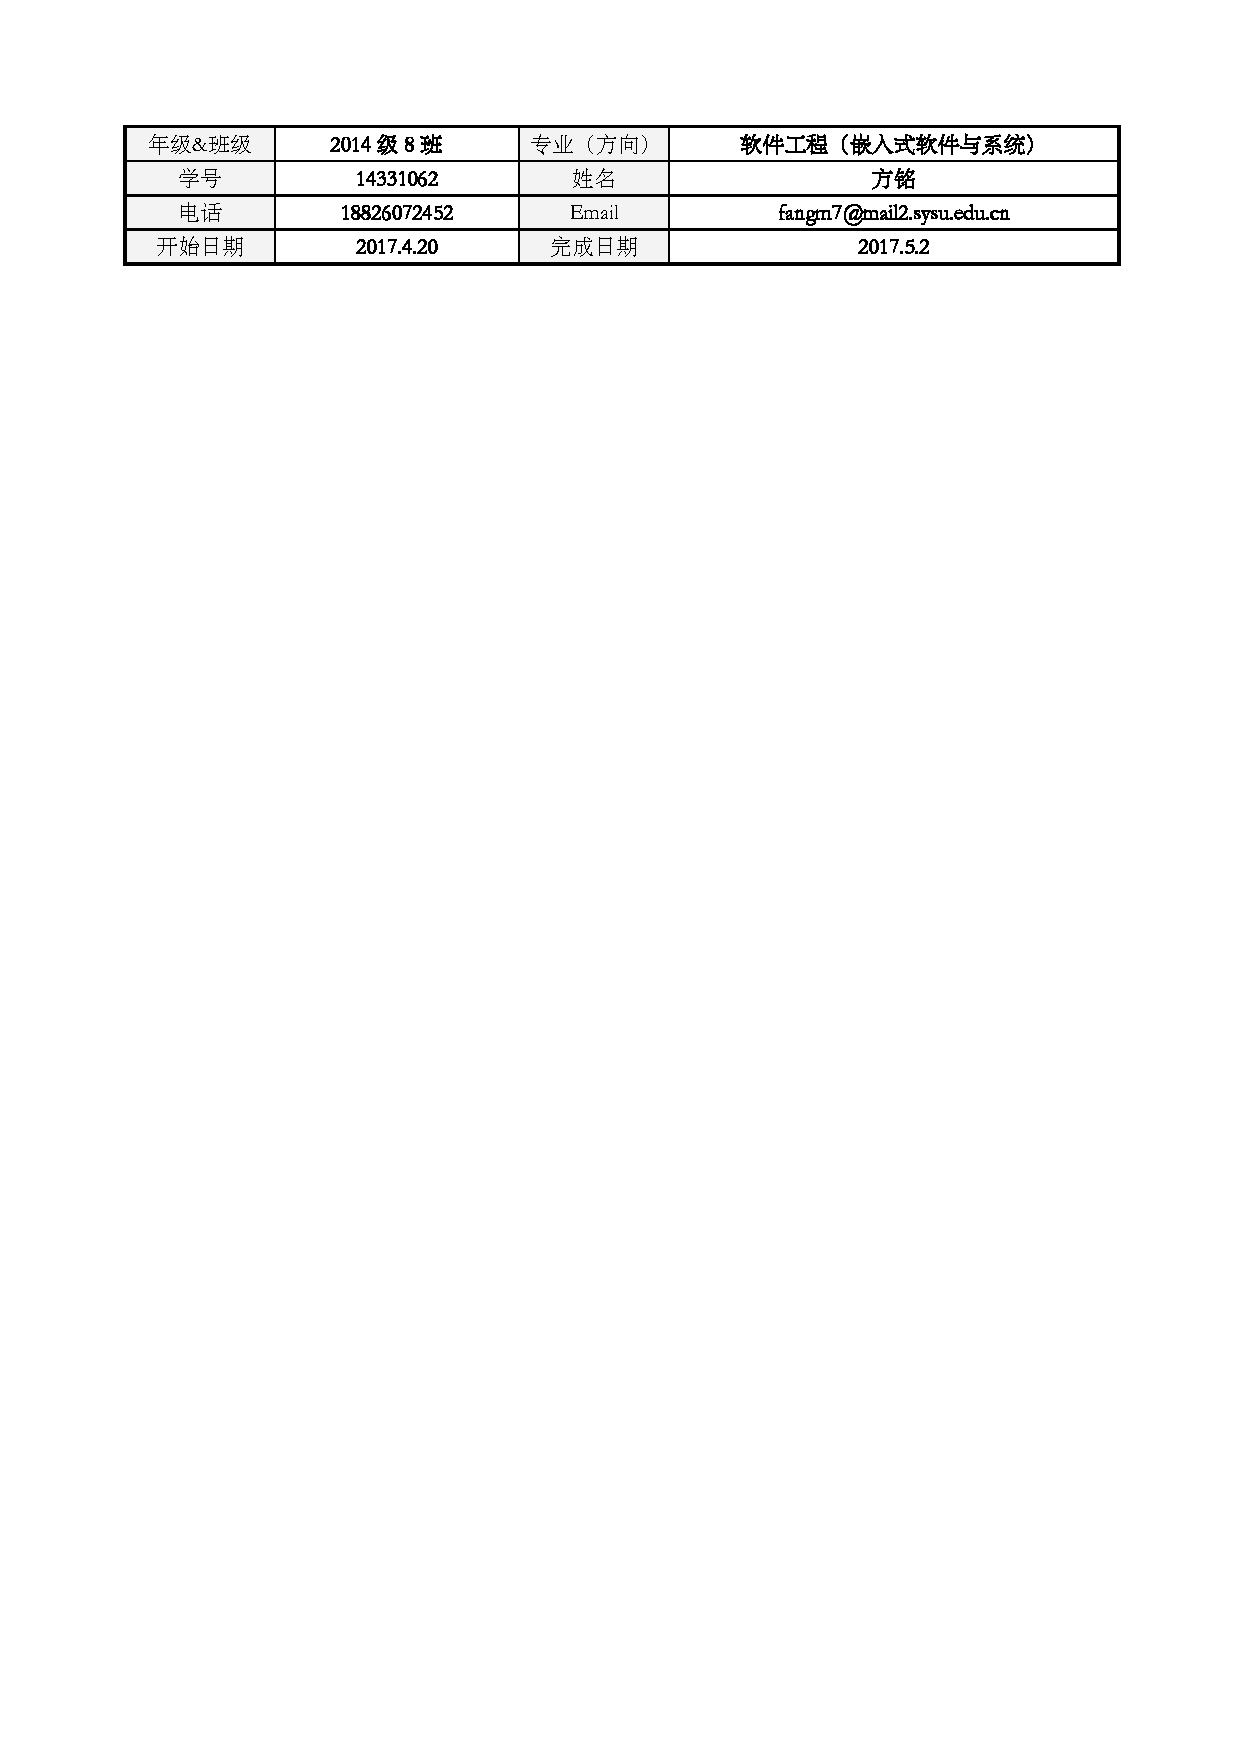
\includegraphics[width=\textwidth]{figure/info.pdf}
  \end{flushleft}

  {\noindent\bf\kaiti 实验题目:\palatino Case 1:Pipeline Processor with Hazards
  }

  \section{实验目的}
  \par 在上一次的实验基础上实现带处理Hazard功能的流水线CPU

  \section{实验内容}
  \subsection*{实验步骤}
  \begin{enumerate}
    \item 分析并设计处理器的数据通路和控制通路。
    \item 编写设计代码并编译。
    \item 软件仿真。
    \item 进行硬件配置。
  \end{enumerate}

  \subsection*{实验原理}
  Hazard
  \begin{enumerate}
    \item Structure
    \item Data
    \begin{enumerate}
      \item Arithmetic
      \begin{itemize}
        \item Software solution
        \begin{itemize}
          \item insert NOP
        \end{itemize}
        \item Hardware solution
        \begin{itemize}
          \item Data forwarding
        \end{itemize}
      \end{itemize}
      \item LOAD
    \end{enumerate}
    \item Control
    \begin{itemize}
      \item Software solution
      \begin{itemize}
        \item NOP
        \item Independent operation
      \end{itemize}
      \item Hardware solution\begin{itemize}
        \item Flushing
      \end{itemize}
    \end{itemize}
  \end{enumerate}

\begin{figure}
  \centering
  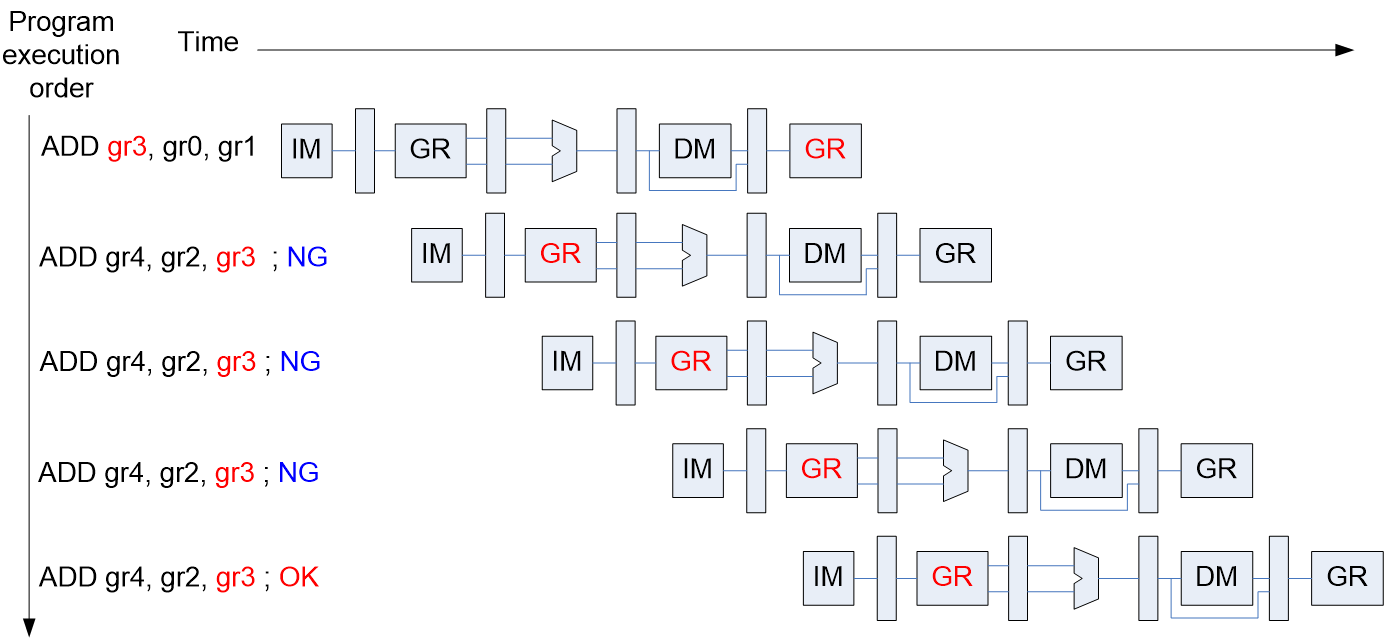
\includegraphics[width=0.8\textwidth]{figure/DataHazards.png}
  \caption{An instruction depends on completion of data access by a previous instruction}
\end{figure}
\begin{figure}
  \centering
  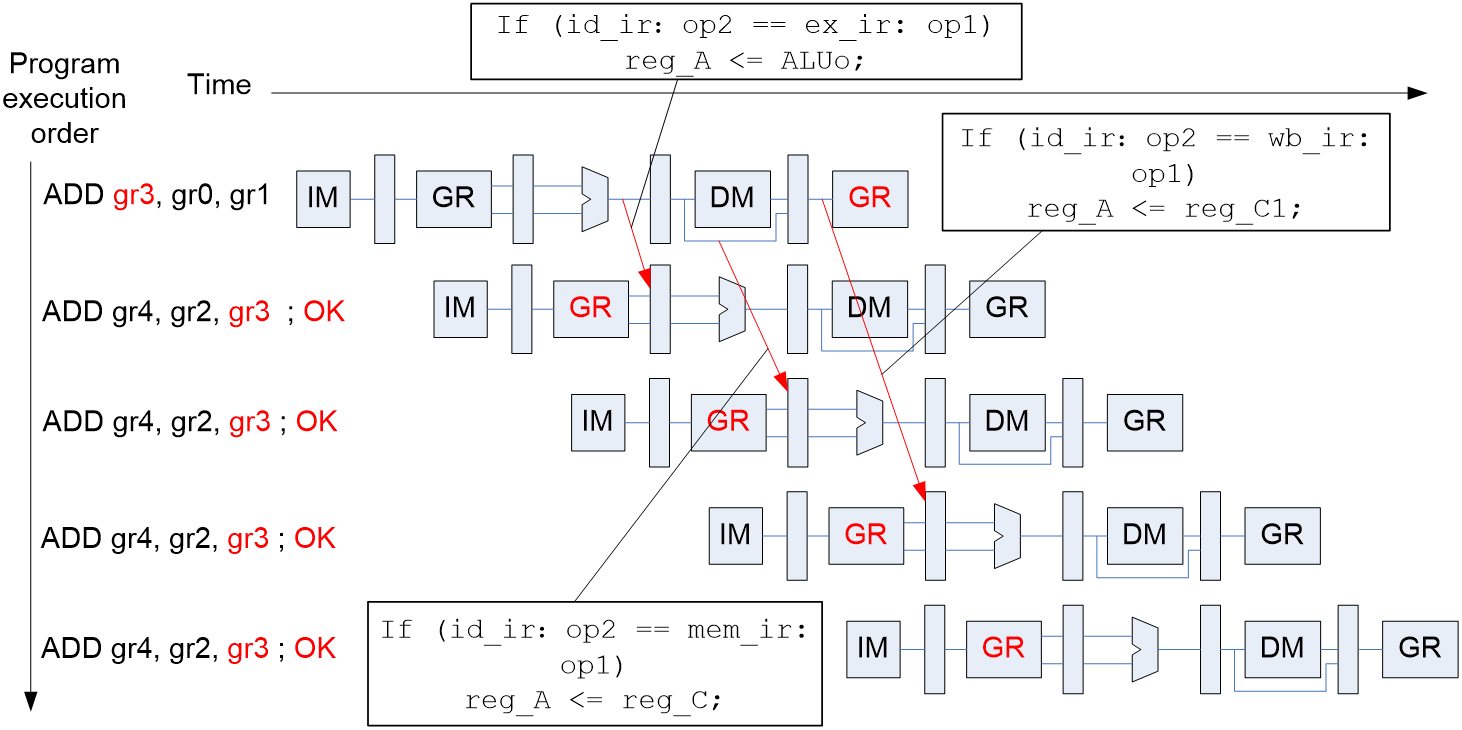
\includegraphics[width=0.8\textwidth]{figure/DataForwarding.png}
  \caption{Data forwarding happens in ID stage, always check id\_ir to decide reg\_A/B}
\end{figure}
\begin{figure}
  \centering
  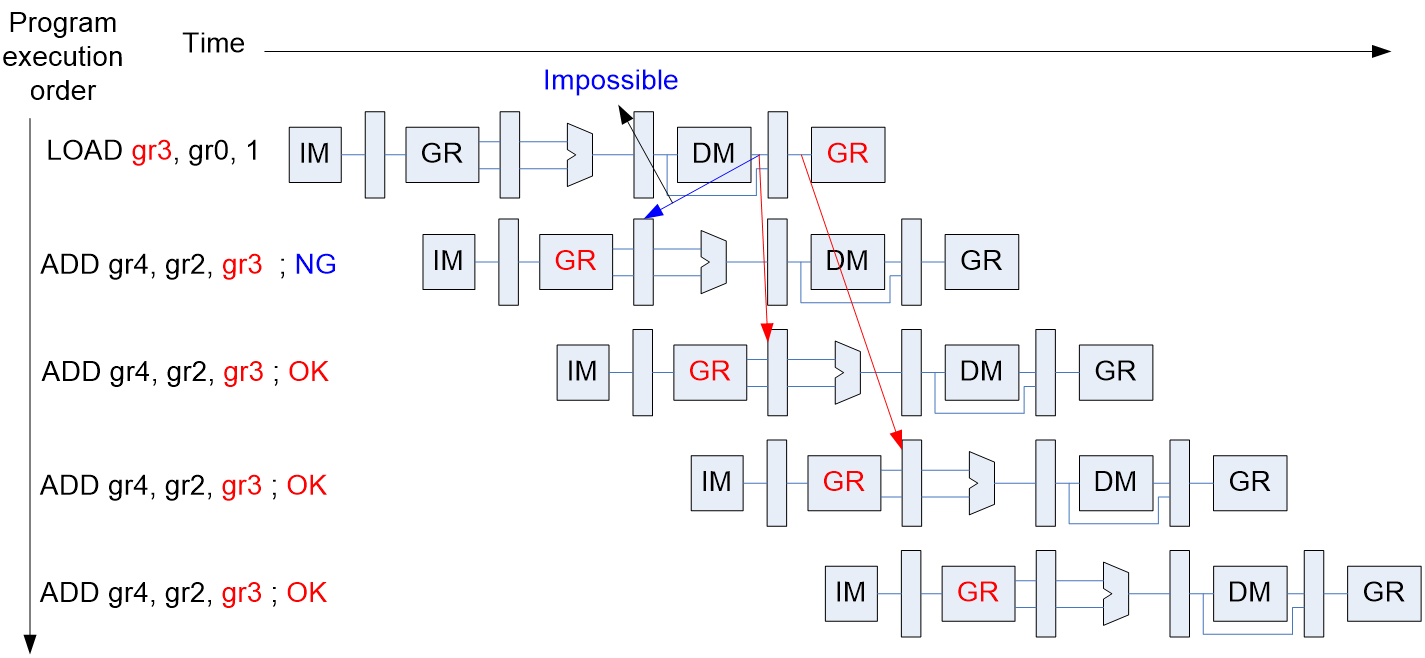
\includegraphics[width=0.8\textwidth]{figure/LoadMiss.png}
  \caption{``LOAD'' can still cause hazard}
\end{figure}
\begin{figure}
  \centering
  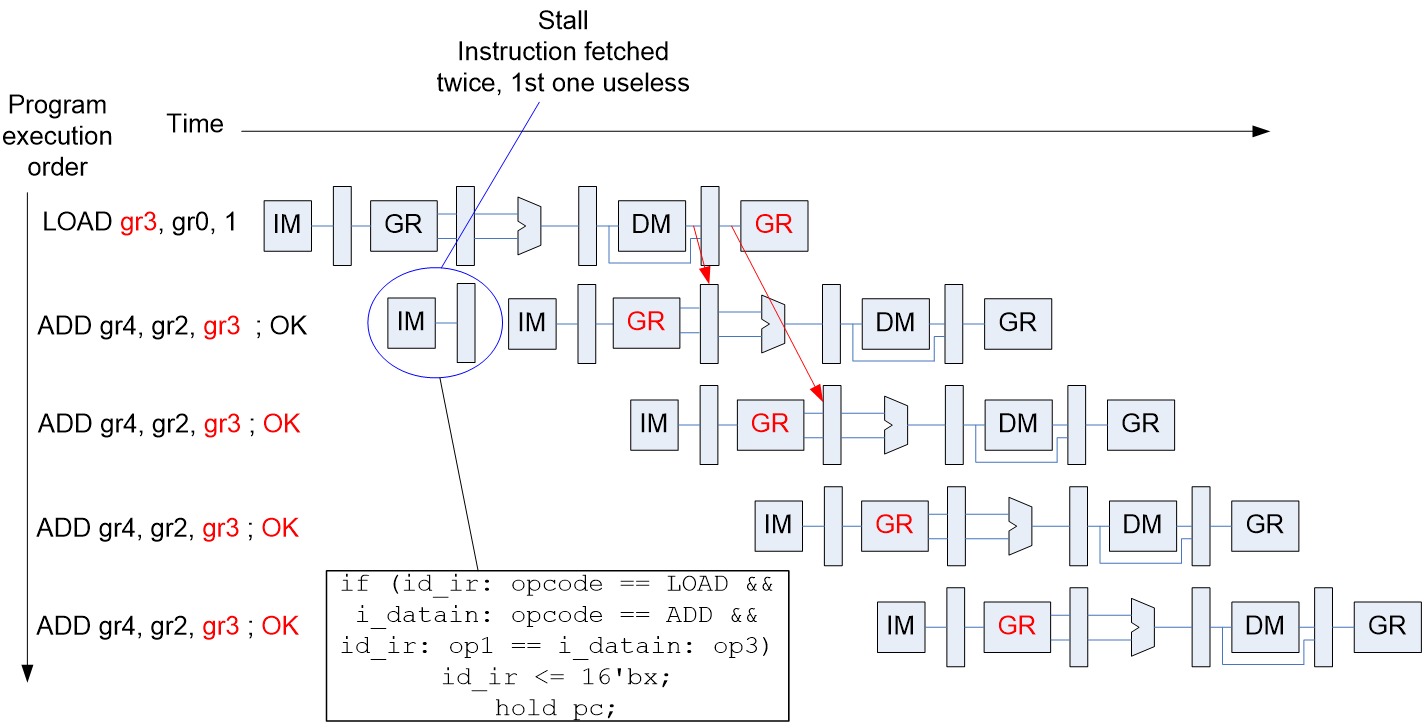
\includegraphics[width=0.8\textwidth]{figure/Stall.png}
  \caption{Stall the pipeline by keeping an instruction in the same stage}
\end{figure}

\subsection*{实验假设}
\begin{enumerate}
  \item 本实验不实现自启动的控制电路,也不提供进程切换所需引脚,不实现进程切换,读、写、内部寄存器的功能。
  \item 开机后pc初始化为0。
  \item 指令和数据有两个独立的缓存,同时读写不会有冲突。
  \item 指令地址和数据地址均已经被映射到缓存(cache)中,读写可在一个时钟周期内完成,从而满足流水线的要求。
  \item 所有通用寄存器在开机或者复位后会清零。
  \item 本实验运行的时钟频率较低,是为了在实验板(Xlinx$^{\textregistered}$ Spartan6 XC6LX16-CS324)上观察调试。可以在实验板上正常工作的最大时钟频率暂未测定。
\end{enumerate}

  \section{实验结果}
\subsection{综合的RTL电路图}
增加hazard处理后的PCPU模块的RTL图见附录。

\subsection{texture simulation}
\subsubsection{简单指令测试}
内存初始值:
\begin{flushleft}
  \begin{minipage}{0.3\textwidth}
    \lstinputlisting[language=PlainText]{code/def_d_mem.txt}
  \end{minipage}
\end{flushleft}
\newpage
\par {\bf Testing LOAD/STORE hazard}
\begin{figure}[H]
  \begin{minipage}{0.3\textwidth}
    测试代码 load.asm
    \lstinputlisting[language=Assembler,firstnumber=0]{code/load.asm}
  \end{minipage}
  \hspace{1em}
  \begin{minipage}{0.65\textwidth}
    \centering
    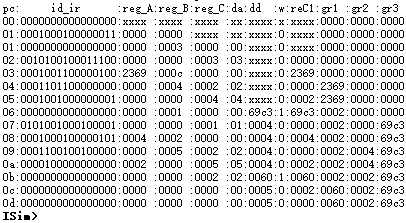
\includegraphics[width=\textwidth]{figure/simu/loadtest.png}
    \caption{pc is stalled when pc = 1 and  data are correctly forwarded}
  \end{minipage}
\end{figure}
\par 这里测试了从内存读取数据后,马上使用该数据的情况。
容易忽视store指令的R1寄存器也可能存在数据冒险情况。
指令8测试了同时存在两个数据冒险的情况。
\par
通过对比,可以看到添加nop指令(指令5)对pc值的影响:
pc=1时维持了2个时钟,而pc=5时只维持了一个时钟。
如果从内存load一个数,并立即通过store写回内存,那么不需要阻塞 pc,
可以通过数据旁路获得数值。

\par {\bf Testing data hazard}
\begin{figure}[H]
  \begin{minipage}{0.28\textwidth}
    测试代码 consecutivedata.asm
    \lstinputlisting[language=Assembler,firstnumber=0]{code/consecutivedata.asm}
  \end{minipage}
  \hspace{1em}
  \begin{minipage}{0.65\textwidth}
    \centering
    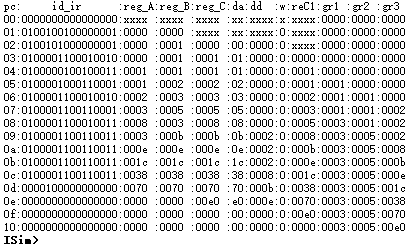
\includegraphics[width=\textwidth]{figure/simu/datatest.png}
    \caption{all data are correctly forwarded}
  \end{minipage}
\end{figure}

\par 这里重点测试了数据旁路。
\par 指令2-6测试了两个操作数同时需要旁路的情况。
\par 指令6-11测试了多次更新某个通用寄存器时旁路的优先级,应该从最近被修改的寄存器那里获取数值。

\par {\bf Testing branch hazard}
\begin{figure}[H]
  \centering
  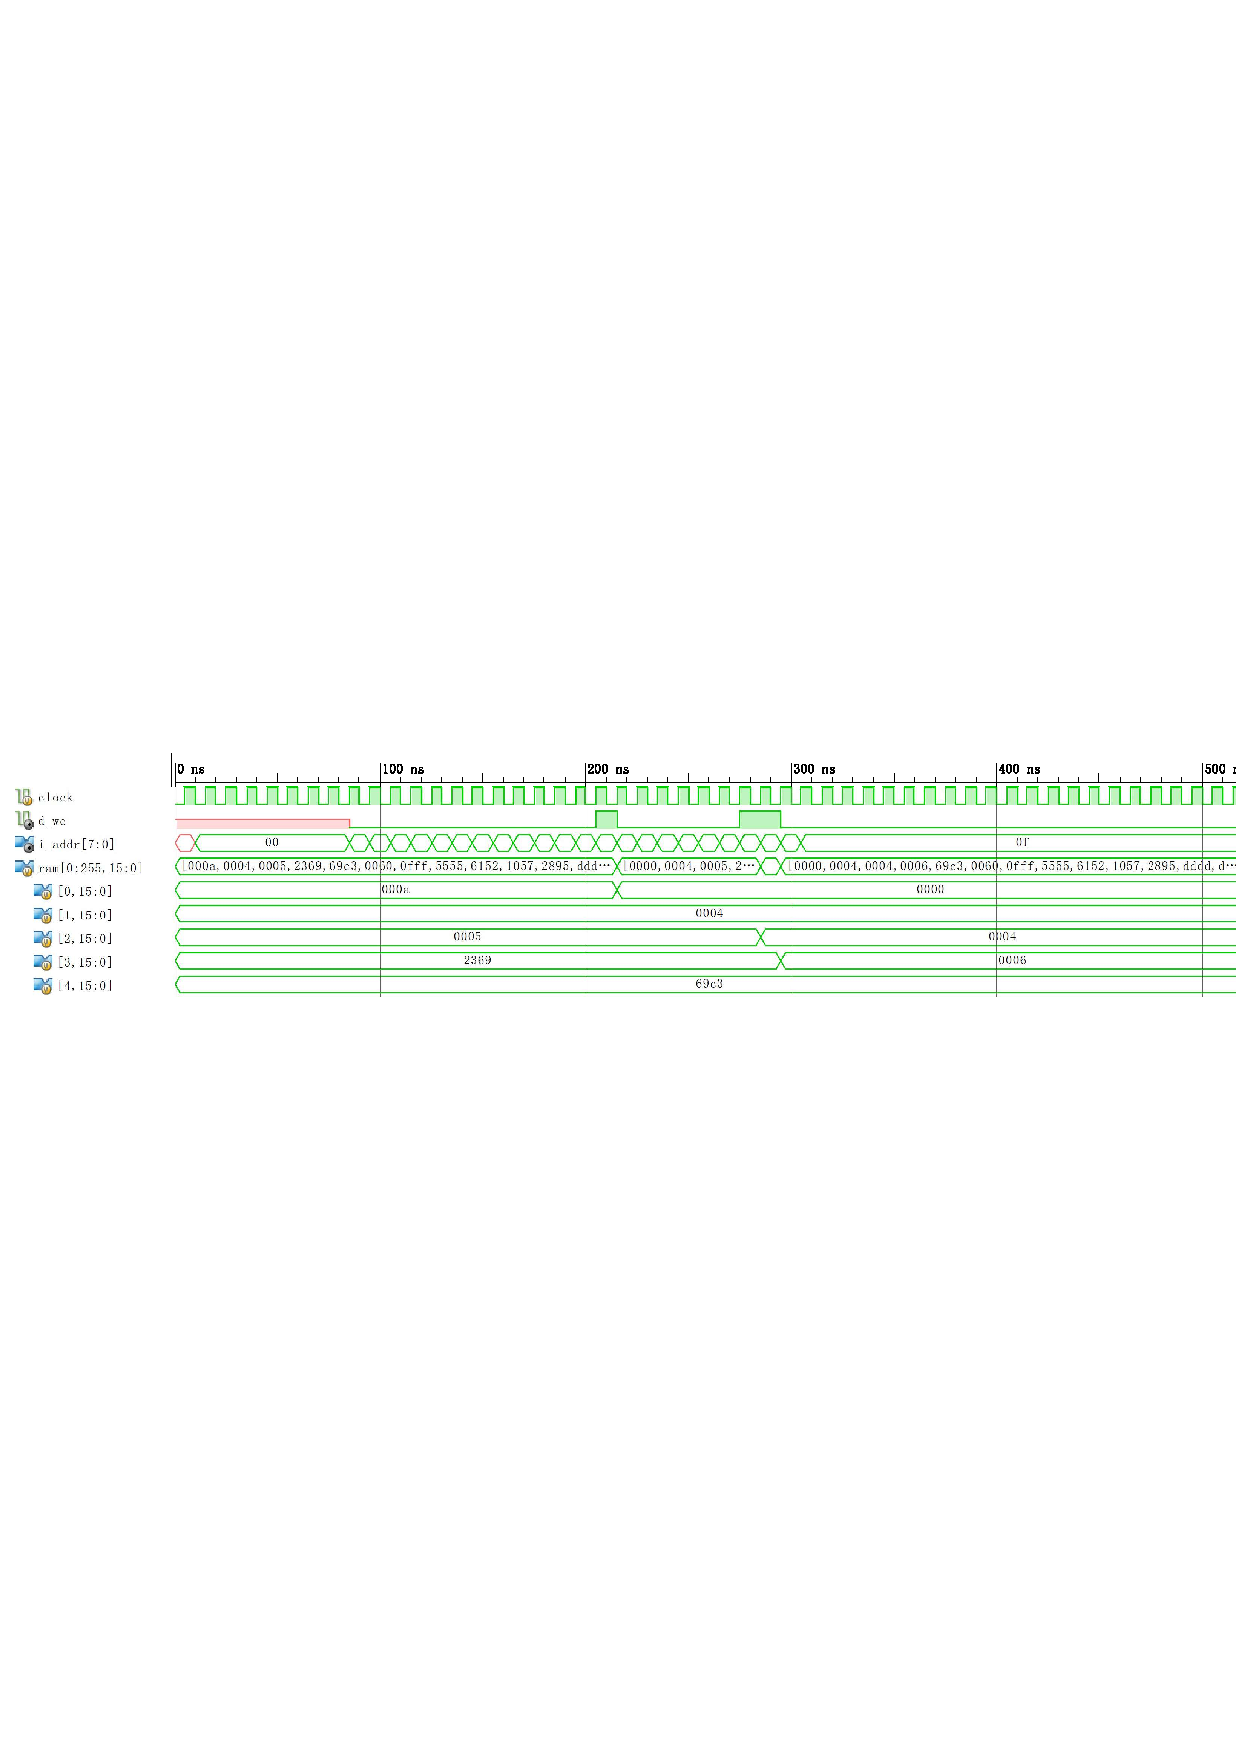
\includegraphics[width=\textwidth]{figure/simu/branchmemwave.pdf}
  \caption{前三个地址单元的内存读写波形图}
  \label{Fig.memwave}
\end{figure}
\begin{figure}[H]
  \begin{minipage}{0.32\textwidth}
    测试代码branch.asm
    \lstinputlisting[language=Assembler,firstnumber=0]{code/branch.asm}
  \end{minipage}
  \hspace{1em}
  \begin{minipage}{0.65\textwidth}
    \centering
    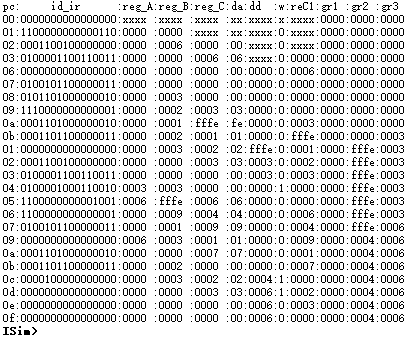
\includegraphics[width=\textwidth]{figure/simu/branchtest.png}
    \caption{flush when branch predict is wrong}
  \end{minipage}
\end{figure}
\par 这里重点测试了跳转后是否存在对涉及通用寄存器和数据内存的非法写入,以及有没有非法的跳转(指令5)。
经测试,跳转后没有非法的写入操作,指令5也没有真正被执行。第二次执行指令9时,因为没有成功跳转,所以不需要清除流水线。
内存读写波形图见图\ref{Fig.memwave}。

\par {\bf Testing halt}
\begin{figure}[H]
  \begin{minipage}{0.4\textwidth}
    测试代码halt.asm
    \lstinputlisting[language=Assembler,firstnumber=0]{code/halt.asm}
  \end{minipage}
  \hspace{1em}
  \begin{minipage}{0.55\textwidth}
    \centering
    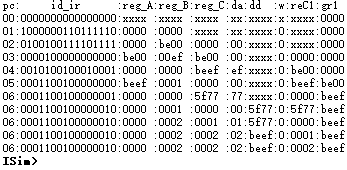
\includegraphics[width=\textwidth]{figure/simu/halttest.png}
    \caption{halt}
  \end{minipage}
\end{figure}
\par 对于流水线CPU,一条指令需要分多个阶段执行,因此取指导停机指令后还不能立即停下。
如果halt指令后没有写加上三个nop,在装入指令寄存器之后,由于指令内存可能未初始化为0,
halt后可能跟有store,涉及到对数据内存的写入操作,破坏原始数据。因此要禁止在halt后对内存的写操作。
这里重点测试了halt指令后,是否存在对数据内存的非法写入。由于写回操作是最后一个阶段,
肯定在halt指令完全经过流水线之后,因此一般通用寄存器不会被修改。

\subsubsection{复杂指令测试}
\indent\par {\bf sort}
\par 测试代码及初始内存见附录,运行结束后,数据内存的结果如下:
\begin{figure}[H]
  \centering
  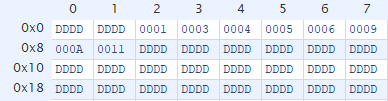
\includegraphics[width=0.5\textwidth]{figure/simu/advance/sort.png}
  \caption{数据内存的结果}
\end{figure}

\par {\bf inst\_test}
\par 测试代码及初始内存见附录,运行结束后,数据内存的结果如下:
\begin{figure}[H]
  \centering
  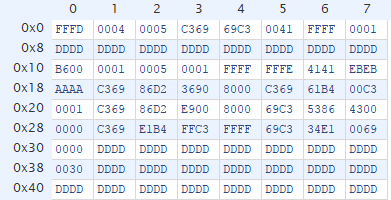
\includegraphics[width=0.5\textwidth]{figure/simu/advance/inst.png}
  \caption{数据内存的结果}
\end{figure}
\par 这里未定义的内存初始化为0xdddd。运行结果除了地址为0x5的内存单元外,与复杂指令测试【origin】中得dmem.mem.master的结果完全一致。
与《测试结果.doc》不一致的内存单元有0x23,0x26,0x27,0x28,这部分涉及的指令是sla,我实现的方式是
{\consolas ALUo = \{operand[15], operand[14:0] << shift\}}, 估计《测试结果.doc》所采用的实现方式是
{\consolas ALUo = \$signed(operand) <<< shift }, 因此会有不同。实际上,
{\consolas \$signed(operand) <<< shift = operand << shift}。我更倾向于算术左移操作保留符号位,等价于算术上乘以2,
因此在这里保留不同结果。

\par {\bf gcd\&lcm}
\par 测试代码及初始内存见附录,运行结束后,数据内存的结果如下:
\begin{figure}[H]
  \centering
  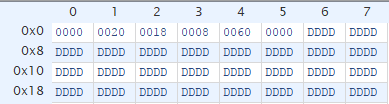
\includegraphics[width=0.5\textwidth]{figure/simu/advance/gcdlcm.png}
  \caption{数据内存的结果}
\end{figure}
\par 这个程序是求:数字0x20和数字0x18的最大公约数和最小公倍数。最大公约数求出是  0x0008,最小公倍数是0x0060。

\par {\bf add64b}
\par 测试代码及初始内存见附录,运行结束后,数据内存的结果如下:
\begin{figure}[H]
\hspace{1em}
\begin{minipage}{0.25\textwidth}
\consolas
\begin{tabular}{rr}
  &0000 FFFE FFFE FFFE\\
 +&0000 FFFF FFFF FFFF\\
 \hline
  &0001 FFFE FFFE FFFD\\
\end{tabular}
\end{minipage}
\begin{minipage}{0.7\textwidth}
  \centering
  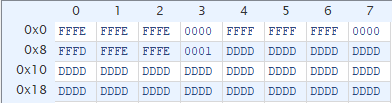
\includegraphics[width=0.714\textwidth]{figure/simu/advance/add64b.png}
  \caption{数据内存的结果}
\end{minipage}
\end{figure}
\par 0x0-0x3为被加数,0x4-0x7为加数,0x8-0xb为求和结果。三个64位整数都是按小端模式(Little-Endian)存放。

\par {\bf bubble}
\par 测试代码及初始内存见附录,运行结束后,数据内存的结果如下:
\begin{figure}[H]
  \centering
  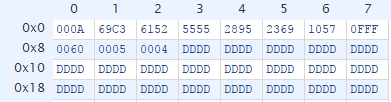
\includegraphics[width=0.5\textwidth]{figure/simu/advance/bubble.png}
  \caption{数据内存的结果}
\end{figure}
\par 0x0单元表示有10个数要排序。运行完后,数据已经有序的(降序)。

\subsection{开发板的显示效果}
\begin{itemize}
  \item SW7为Debug,0表示选择自动时钟,1为选择手动时钟,按下并释放中间的BTN(B8)可以让手动时钟翻转一次;
  \item SW6为enable,SW5为start,若要使能并开始运行,需要把这两个开关打开;
  \item 按下BTNU可以重置CPU,由于我使用IP core生成内存时没有加入RESET功能,所以内存数据不会重置。
  \item SW3-SW0为select[3:0]用于选择在数码管上显示的数据,定义见附录PCPU.v,
  \item SW4为选择显示通用寄存器,当SW4打开时,结合SW2-SW0可以选择0-7号通用寄存器。
\end{itemize}

\par 5个复杂指令测试生成的bit文件以及仿真测试输出的dmem.mem.master文件均已提交至ftp result目录下,
并且已经上传至我的github:\url{https://github.com/SimonFang1/Pipeline-RISC-CPU}。
烧入add64b对应的bit文件,运行程序,运行结束后,通用寄存器的结果显示如下:
\begin{figure}[H]
  \centering
  \foreach \n in {0,...,7} {
    \begin{minipage}{0.45\textwidth}
      \includegraphics[width=\textwidth]{figure/boardresult/\n.jpg}
    \end{minipage}
  }
  \caption{通用寄存器gr[0:7]的最终结果}
\end{figure}

\par 运行结束后,pc和wb\_ir的结果显示如下:
\begin{figure}[H]
  \centering
  \begin{minipage}{0.45\textwidth}
    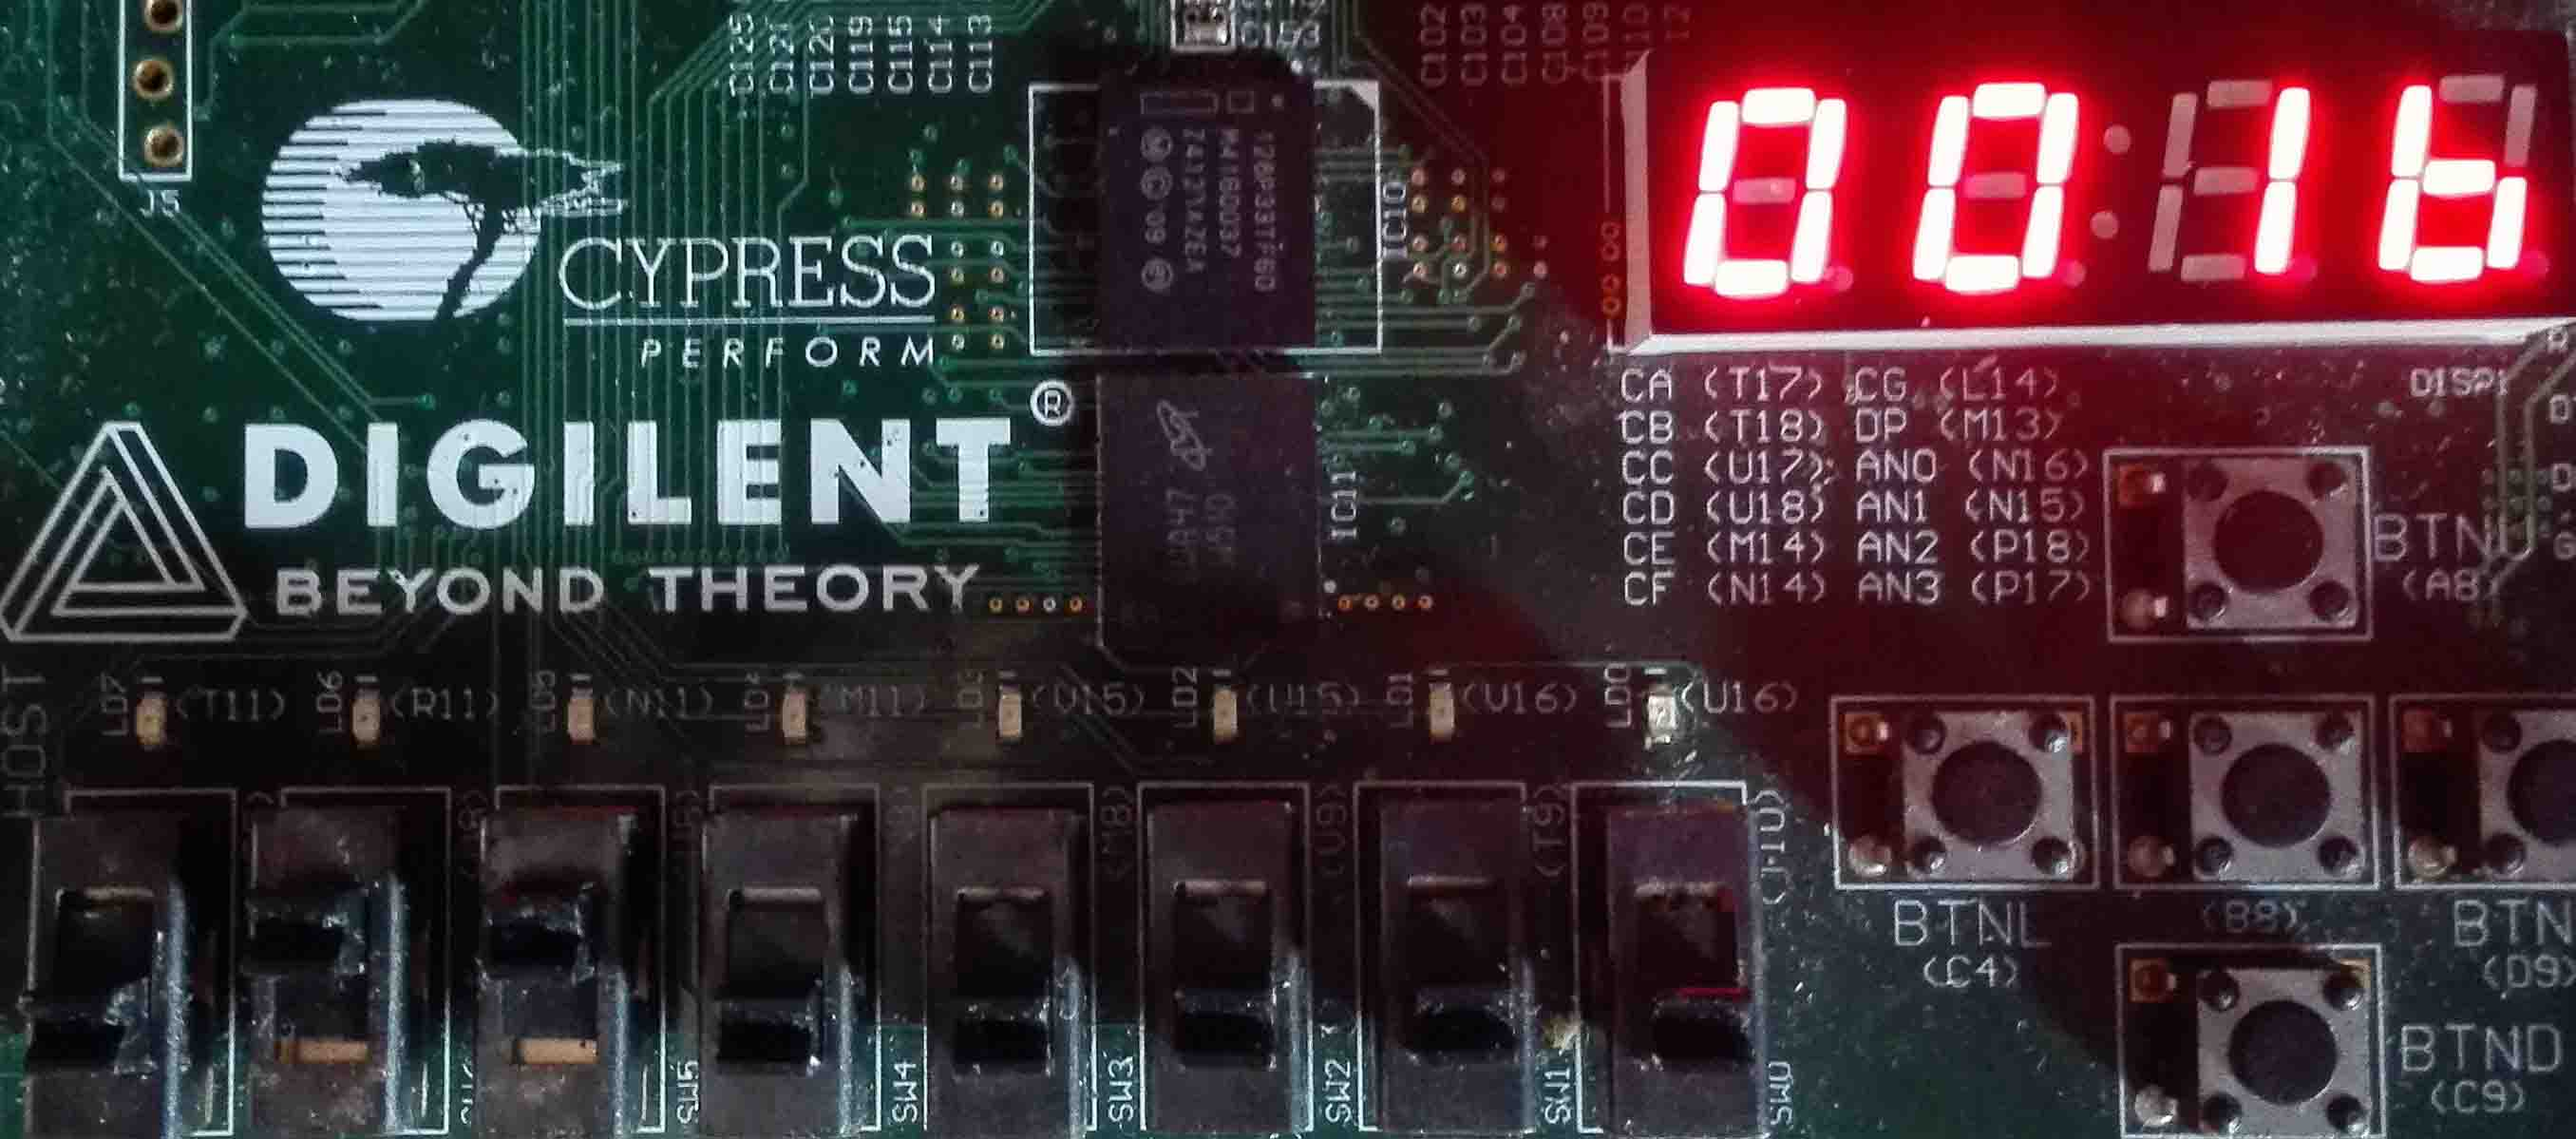
\includegraphics[width=\textwidth]{figure/boardresult/pc.jpg}
    \caption{pc的最终结果}
  \end{minipage}
  \begin{minipage}{0.45\textwidth}
    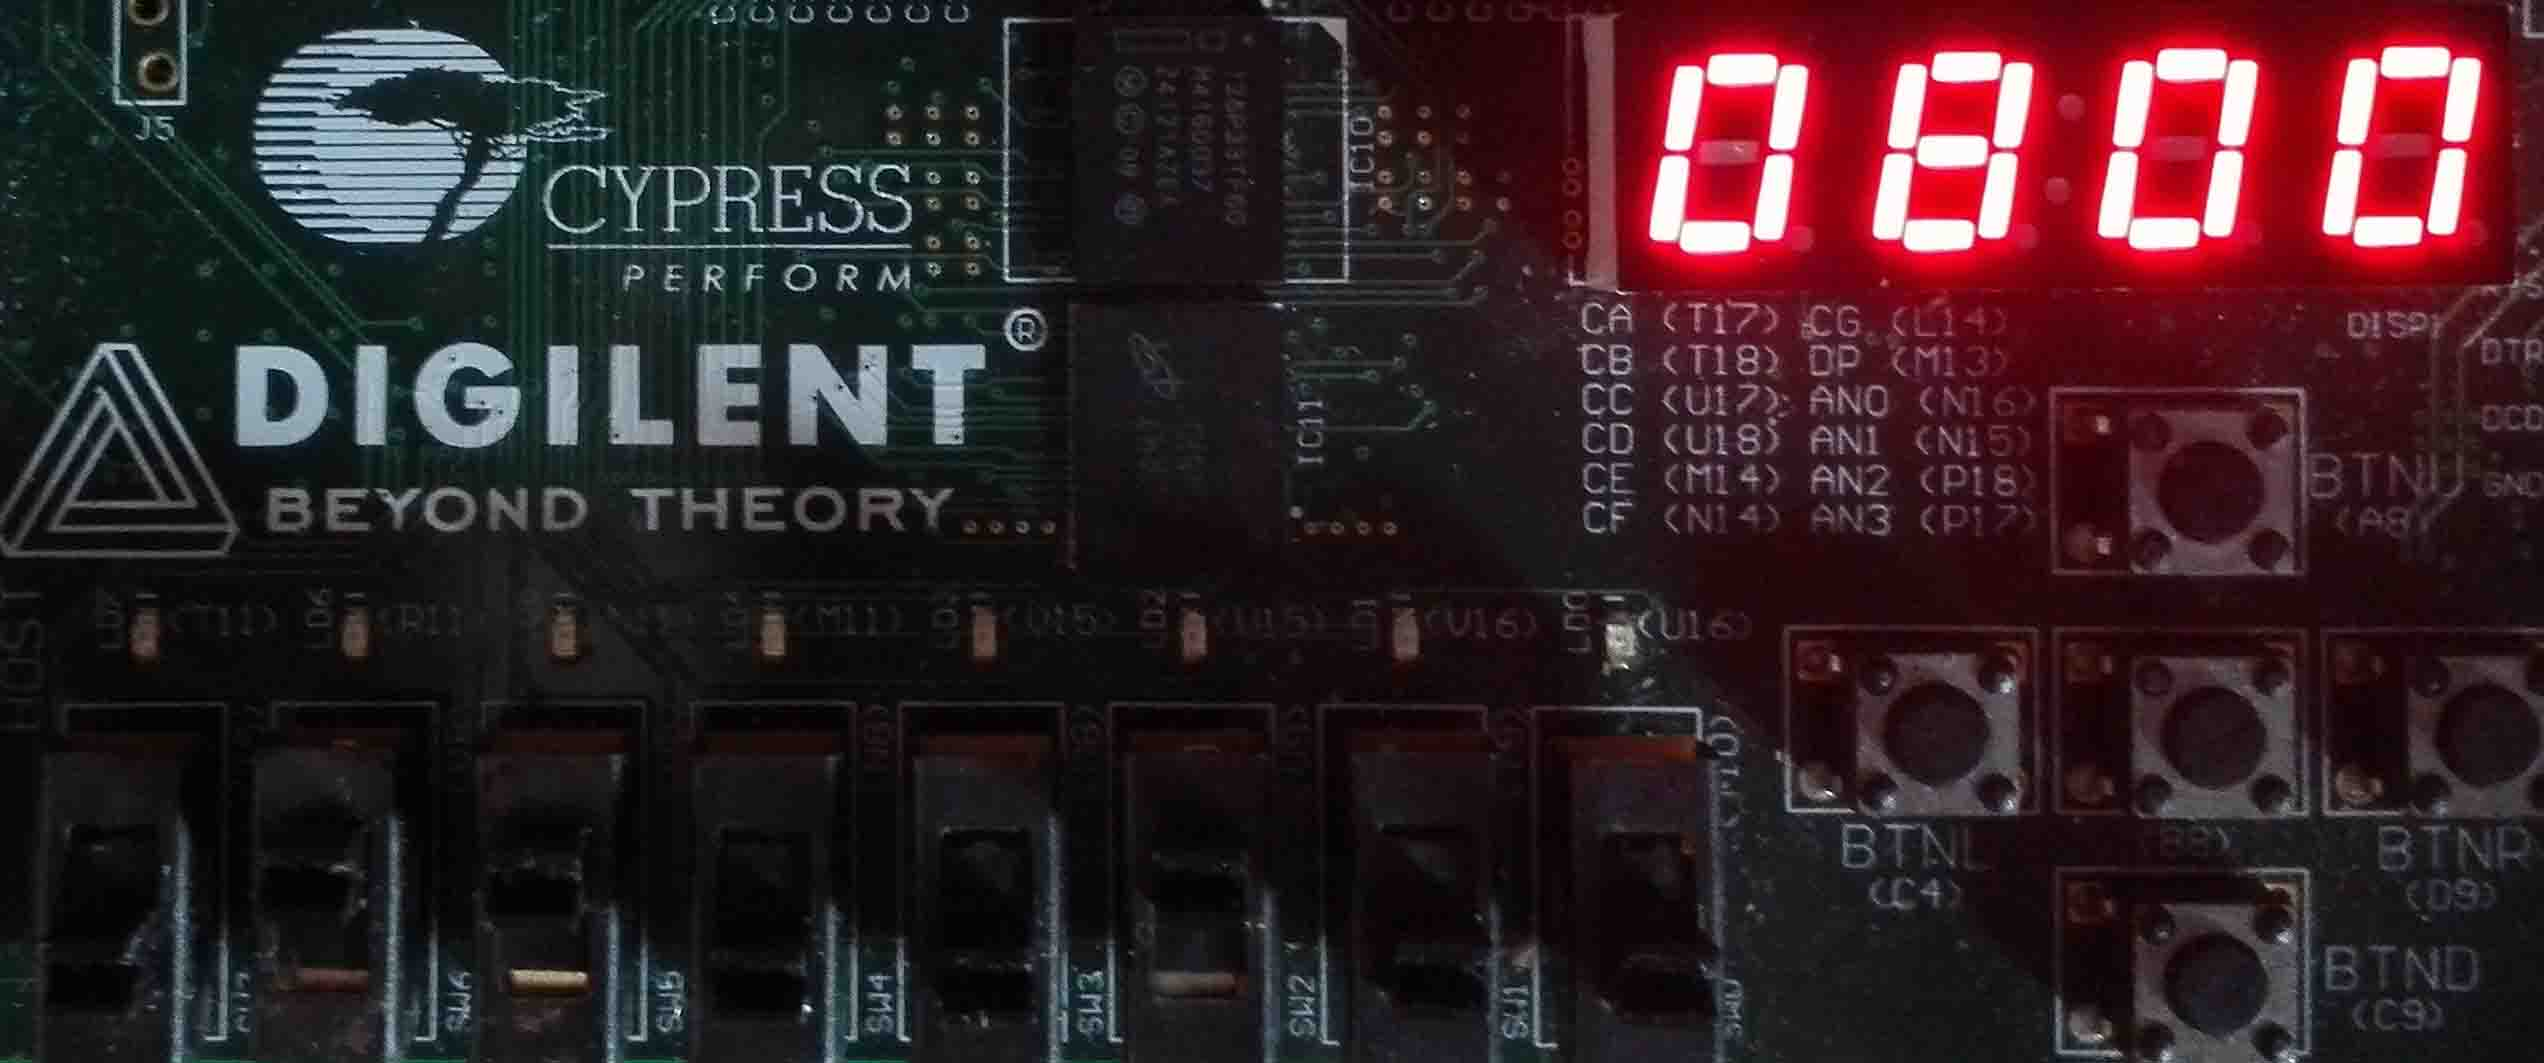
\includegraphics[width=\textwidth]{figure/boardresult/wb.jpg}
    \caption{wb\_ir的最终结果}
  \end{minipage}
\end{figure}

 \section{实验感想}
   \setlength{\parskip}{0.5\baselineskip}
   \par 本次实验实现了一个基于精简指令集的流水线CPU,可以正确有序地执行输入指令,
   经仿真测试和板级综合验证,通过了5个复杂指令测试,进一步提高了我利用verilog语言设计并实现较复杂硬件系统的能力。
   \par 实验实现的CPU具备很弱的分支预测功能,即在发生分支跳转时,也能先把pc+1,pc+2,pc+3的指令先装入流水线,
   对b类型的指令具有一定的分支预测功能,而对j类型的指令则是100\%错误预测率。
   \par 如果要进一步改进流水线CPU,可以增强分支预测的功能。
   支持j(jump)指令的分支预测比较简单。j指令可以在译码阶段获取立即数得到pc下个时钟周期的值。
   j指令没有分支,能做到100\%的正确预测率。
   jr(jmpr)指令需要读取寄存器,也有可能有读取冒险,有不确定性,因此考虑和b类型的指令一起用预测跳转表的值进行预测。
   支持b类型的指令需要若干个预测跳转表,按照最近最少使用(LRU)的原则,为所有的jr指令,b类型的指令分配预测跳转表。
   在取指阶段直接从预测跳转表跳中确定pc下个时钟周期的值,如果缺失,则使用pc+1作为默认值。
   \par 一般情况下,在load指令后需要立即使用寄存器值的话,需要延迟一个时钟周期,但是store指令除外,
   如果需要把某个内存单元的值写到另一个内存单元,那么两个连续的load和store指令执行起来不需要延迟一个时钟。
   但是,如果通过load指令更新了某个寄存器,而这个寄存器的值是store指令寻址的基地址,
   那么两个连续的load和store指令之间还是会有一个延迟。
   \par 本以为通过了inst\_test这一复杂指令测试,其他复杂指令测试应该都能通过。但是通过sort测试,
   出现了不能停机的情况。这是由于更新pc时,没有充分考虑条件判断的优先级,在这个测试中,
   需要通过bz指令进行条件跳转,实际上判断跳转时,bz指令已经进入了mem\_ir,而此时id\_ir的指令是load,
   代取指的指令和load之间存在冒险,需要延迟,pc需要保持不变。如果判断时,后者(stall)的优先级比前者(pc跳转)高,
   就会出现上述无法停机的情况。
   \par 所有涉及到立即数的指令,立即数的表示形式都是无符号整数,
   这是考虑到addi指令需要和ldih指令配合来实现一个16位立即数,如果实现成有符号整数,那么addi的时候就会在高位补0xff,破坏
   ldih所读入的立即数。
   \par 经过实验验证并结合我的分析,我认为:使用always @* 语句生成组合电路时,不完整的条件语句会导致latch,但是always @(posedge clk)结合非阻塞赋值 <= 生成的触发器可以没有完整的条件分支。因为这些语句生成的是触发器,分支中赋值的语句的右值作为数据选择器的输入,判断条件通过编码变成一个个选择信号,如果有不完整的条件分支就需要为触发器加一个使能端,为以上条件使能;如果条件分支完整,那么这个触发器不需要使能端,或者令使能端一直处于使能状态。本实验中,我在设计触发器部分时,由于需要保持原来的数据,条件分支没有写完整,但最后也没有任何warning提示生成了latch;相反在利用always @*设计的组合逻辑部分,如果在某个条件分支里写了类似 x = x这样的代码,即使条件完整,也会有warning提示生成了latch。
   \par 实验中使用了Core\_Gernerate 生成了IP,使用了coe文件初始化内存。根据我的理解,IP可以生成一些高级模块的代码,从而进一步完成更加复杂的设计,比如生成一些浮点运算的模块。这可以帮助设计人员减少开发周期,更加快速地设计一些硬件系统。本实验中指令内存被设计为只读的,而数据内存被设计为可读可写的。
%  \newpage
  \appendix
  \titleformat{\section}{\bf\song}{\thesection}{1em}{}
  \newpage
\section*{附录}
\section{复杂指令测试}
\subsection{init\_test}
{
\setlength{\columnsep}{5em}
\begin{multicols}{2}
\par 测试指令
\lstinputlisting[language=Assembler,firstnumber=0]{code/inst_test/code.asm}
\par 初始内存,未指定地址的默认值为0xdddd
\lstinputlisting[language=PlainText]{code/inst_test/def_d_mem.txt}
\end{multicols}
}
\subsection{gcd \& lcm}
{
\setlength{\columnsep}{5em}
\begin{multicols}{2}
\par 测试指令
\lstinputlisting[language=Assembler,firstnumber=0]{code/gcdlcm/code.asm}
\par 初始内存,未指定地址的默认值为0xdddd
\lstinputlisting[language=PlainText]{code/gcdlcm/def_d_mem.txt}
\end{multicols}
}
\subsection{add64b}
{
\setlength{\columnsep}{5em}
\begin{multicols}{2}
\par 测试指令
\lstinputlisting[language=Assembler,firstnumber=0]{code/add64b/code.asm}
\par 初始内存,未指定地址的默认值为0xdddd
\lstinputlisting[language=PlainText]{code/add64b/def_d_mem.txt}
\end{multicols}
}
\subsection{bubble}
{
\setlength{\columnsep}{5em}
\begin{multicols}{2}
\par 测试指令
\lstinputlisting[language=Assembler,firstnumber=0]{code/bubble/code.asm}
\par 初始内存,未指定地址的默认值为0xdddd
\lstinputlisting[language=PlainText]{code/bubble/def_d_mem.txt}
\end{multicols}
}
\subsection{sort}
{
\setlength{\columnsep}{5em}
\begin{multicols}{2}
\par 测试指令
\lstinputlisting[language=Assembler,firstnumber=0]{code/sort/code.asm}
\par 初始内存,未指定地址的默认值为0xdddd
\lstinputlisting[language=PlainText]{code/sort/def_d_mem.txt}
\end{multicols}
}
\section{设计代码}
其他模块见上次的实验报告,这次改动不大,可以到项目主页
\url{https://github.com/SimonFang1/Pipeline-RISC-CPU}去查看,这里只贴出PCPU.v文件:
\lstinputlisting[language=verilog]{code/PCPU.v}
\section{RTL图}
\newpage
\newgeometry{left=0.4cm,right=0.4cm,top=0cm,bottom=0cm}
\thispagestyle{empty}
\begin{figure}[H]
  \centering
  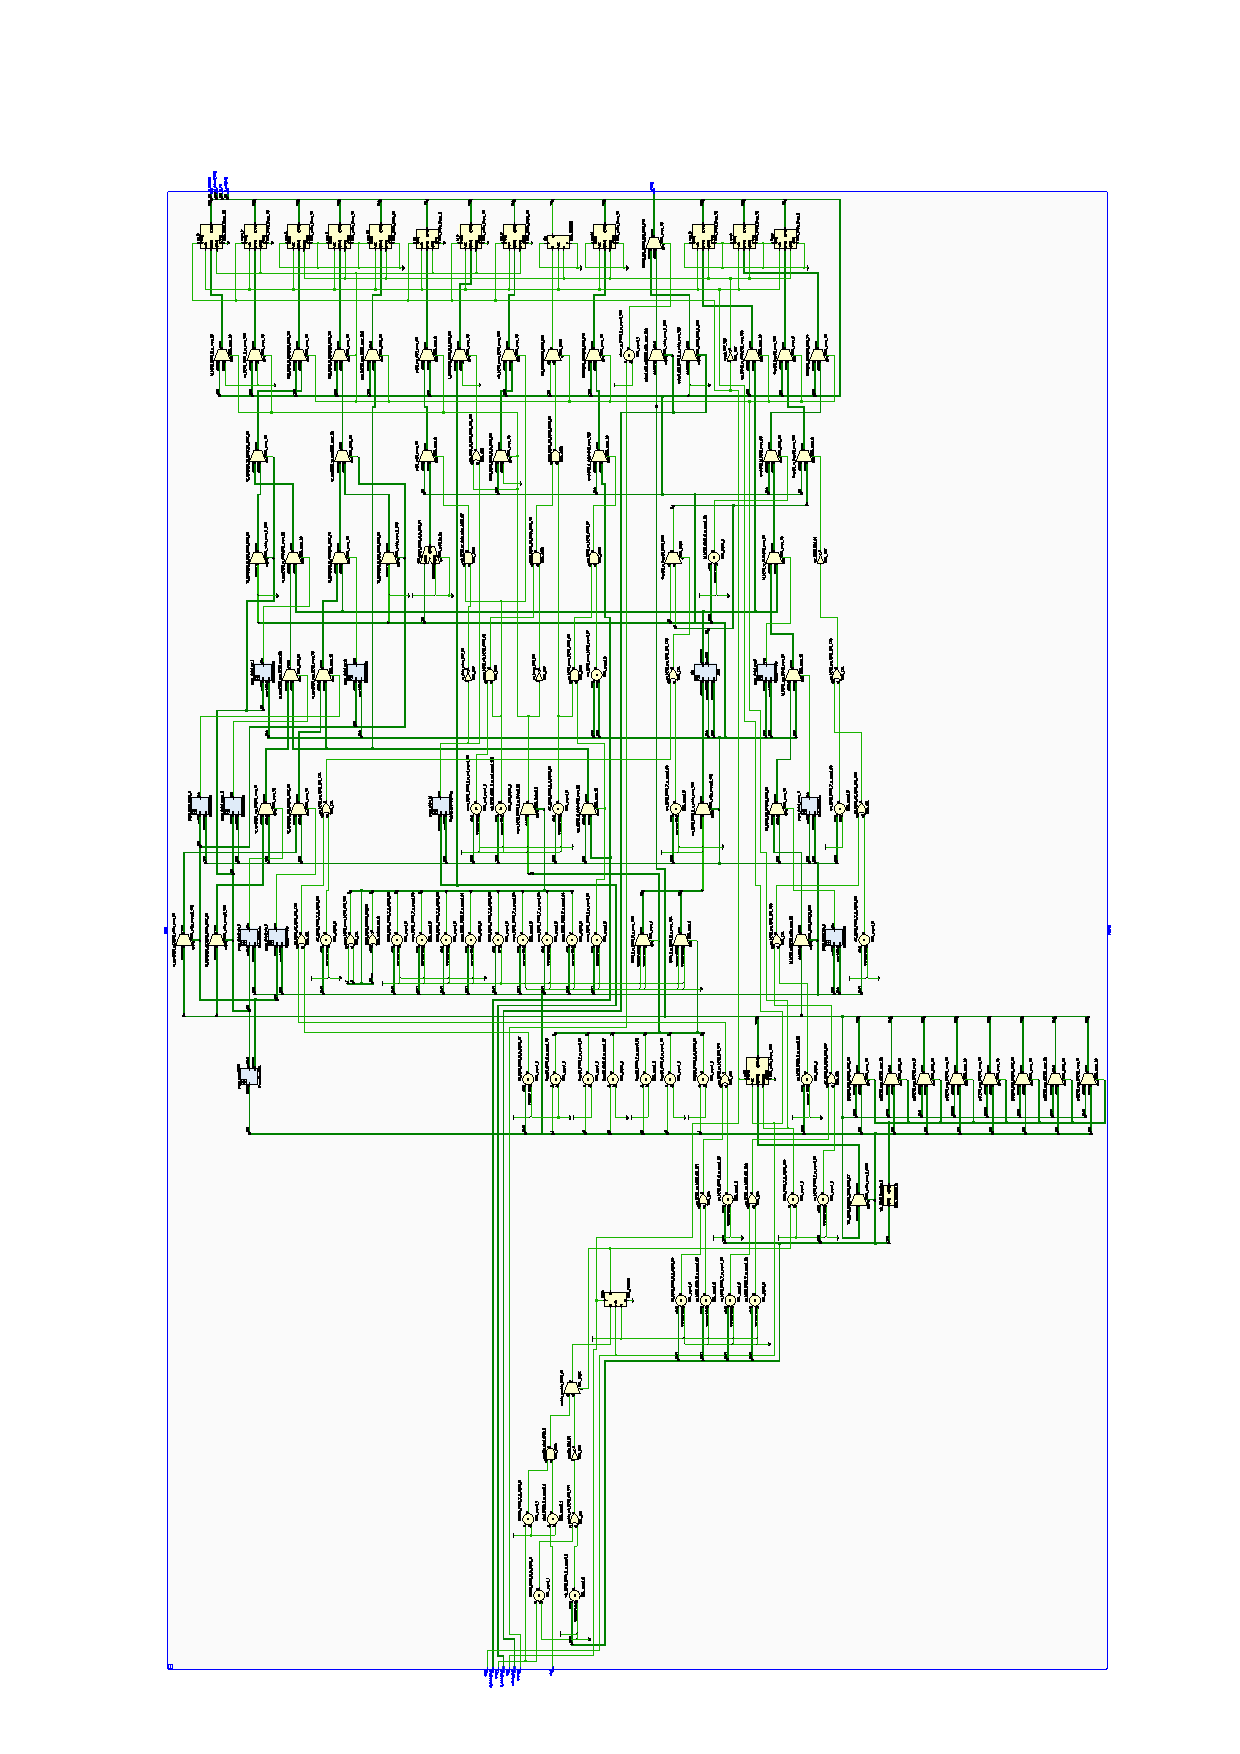
\includegraphics[width=0.9\textwidth]{figure/pcpu.pdf}
  \vspace{-0.8cm}
  \caption{PCPU模块的RTL图(Xilinx PlanAhead 14.7导出)}
\end{figure}
\newpage
\restoregeometry
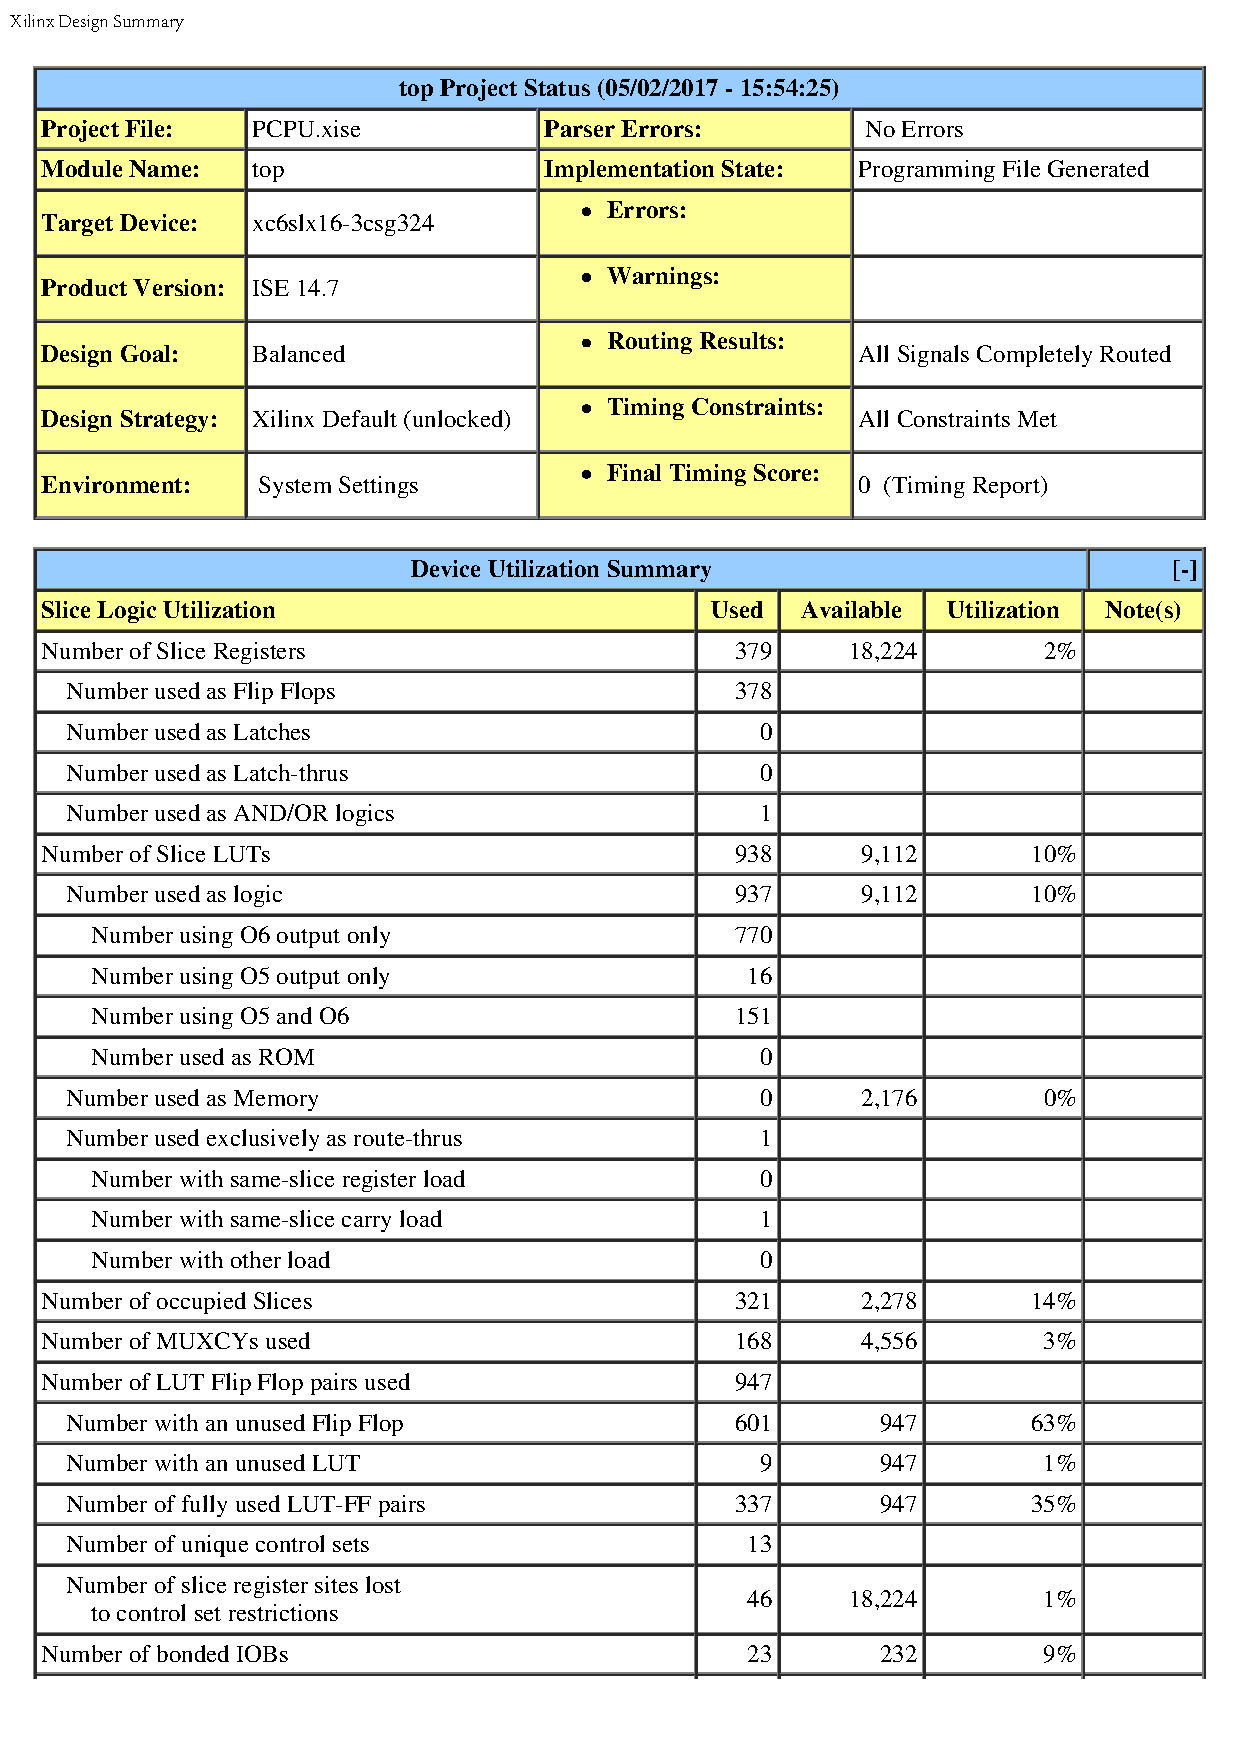
\includepdf[pages=1-2]{top_summary.pdf}
\end{document}
